\chapter{Query Optimization Overview}

In this chapter, we describe the design of cost-based transformational query optimizer, based on Volcano Framework. \\

Query optimization is probably the most critical component of modern database systems, since the ubiquity of the database system depends on the efficiency with which a user's queries are executed by the system. As queries submitted to the database system by the user using a high-level declarative language do not specify an execution plan, it is the job of the optimizer
to generate a good plan, and query optimization can achieve substantial improvements in runtime and resource usage during execution of the query. \\

Traditionally, query optimizers follow a three step approach \cite{roy2000efficient}:
\begin{itemize}
	\item  Generate all execution plans that are logically equivalent to the user-submitted query.
	\item Estimate the cost of executing each of the alternate plans.
	\item Search through the space of all generated plans to find the plan with least cost.
\end{itemize}

\section{Space of Logically Equivalent Plans}
All plans that compute the same result, having the same properties, as that computed by the original query plan, are called to be logically equivalent to the given query. \\

The parser parses the query to generate a query tree. From the initial query tree, the space of all logically equivalent plans can be generated using transformation rules.

\subsection{Logical Plan Space}
The initial query tree consists of logical operators which are like the relational operators select, project, join, etc, and which do not specify the physical algorithm to be used during actual computation. All logical plans that are equivalent to the initial query plan constitute the logical plan space of the query. \\

The logical plan space can be generated by applying logical transformation rules to operators in the logical plan of the query. The new plans generated are further transformed whenever possible, until no new plans can be generated using the given set of rules.

\subsection{Physical Plan Space}
The logical plan must be converted to a physical plan than can be executed on the database system. The implementation rules define which logical operator may be implemented using which physical algorithm. \\

The physical plan space is generated by applying the implementation rules to all plans in the logical plan space.

\section{Logical Space Generation}
We describe the generation of logical plan space in greater detail. The logical plan space is the set of all semantically equivalent logical plans of the input query.

\begin{defn} 
A Logical Query DAG is a directed acyclic graph whose nodes can be divided into equivalence nodes and operation nodes; the equivalence nodes have only operation nodes as children and operation nodes have only equivalence nodes as children. 
\end{defn}

Given a set of rules, we construct a Logical Query DAG from the given input query and expand the DAG to encompass the space of all equivalent logical plans. For example, the query tree of Figure \ref{fig:joinabc}(a) for the query $(A \bowtie B \bowtie C)$ is initially represented in the LQDAG formulation, as shown in Figure \ref{fig:joinabc}(b). The equivalence nodes are shown as boxes, while the operation nodes are shown as circles. \\

The initial LQDAG is then expanded by applying all possible transformations on every node of the initial LQDAG representing the given query. In the example, suppose the only transformations possible are join associativity and commutativity. Then the plans $(A \bowtie (B \bowtie C))$ and $((A \bowtie C) \bowtie B)$, as well as several plans equivalent to these modulo commutativity can be obtained by transformations on the initial LQDAG of Figure \ref{fig:joinabc}(b). These are represented in the LQDAG shown in Figure \ref{fig:joinabc}(c). For exact algorithm refer to pseudocode of procedure \textsc{ExpandDAG} presented in Figure \ref{fig:expandDAG}.

\begin{figure}[here]
\begin{center}
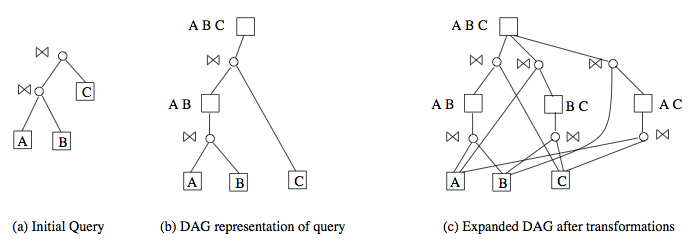
\includegraphics[width=14cm]{Figures/example_logical.png}
\end{center}
\caption{Logical Plan Space Generation for $A \bowtie B\bowtie C$}
\label{fig:joinabc}
\end{figure}

\begin{figure}[here]
\begin{center}
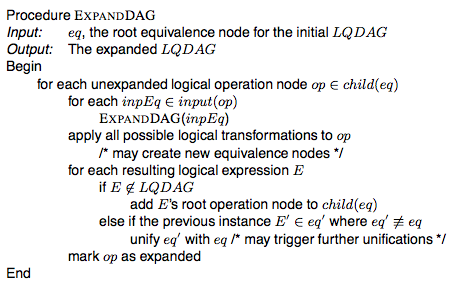
\includegraphics[width=11cm]{Figures/expandDAG.png}
\end{center}
\caption{Algorithm for LQDAG Generation}
\label{fig:expandDAG}
\end{figure}

\section{Cost Model}
The cost of executing a particular physical plan must be estimated for the purpose of finding the optimal plan. As the actual cost is not available during optimization, it is imperative for the estimates to be close to the actual costs in order to find the best plan. \\

The cost model defines how a cost is to be estimated for a particular operator when executed on the database. The optimizer makes use of database statistics, like histograms, and various other rules, for estimating the cost.

\section{Search for Optimal Plan}
The search strategy forms an important part of the optimization scheme. As there are exponentially many alternative plans to be considered, it is infeasible to enumerate all the plans and pick the one with the lowest cost. The optimizer must incorporate pruning techniques to reduce the size of the search space that will be explored during optimization.
